% !TeX root = document.tex
% !TeX encoding = UTF-8 Unicode

\chapter{Floats}
\section{Figuras}

Adicione figuras com o ambiente \texttt{figure} e referencie com \texttt{ref}. A
palavra antes da referência sempre tem inicial maíuscula: Figura~\ref{fig:smm1}.
O til entre Figura e o comando \texttt{ref} é um espaço que não pode ser
quebrado.

\begin{figure}[ht!] % ht! é o posicionamento da figura.
  \centering % centraliza a figura no ambiente figure
  % Ajuste o tamanho da figura usando a porcentagem em frente à \linewidth.
  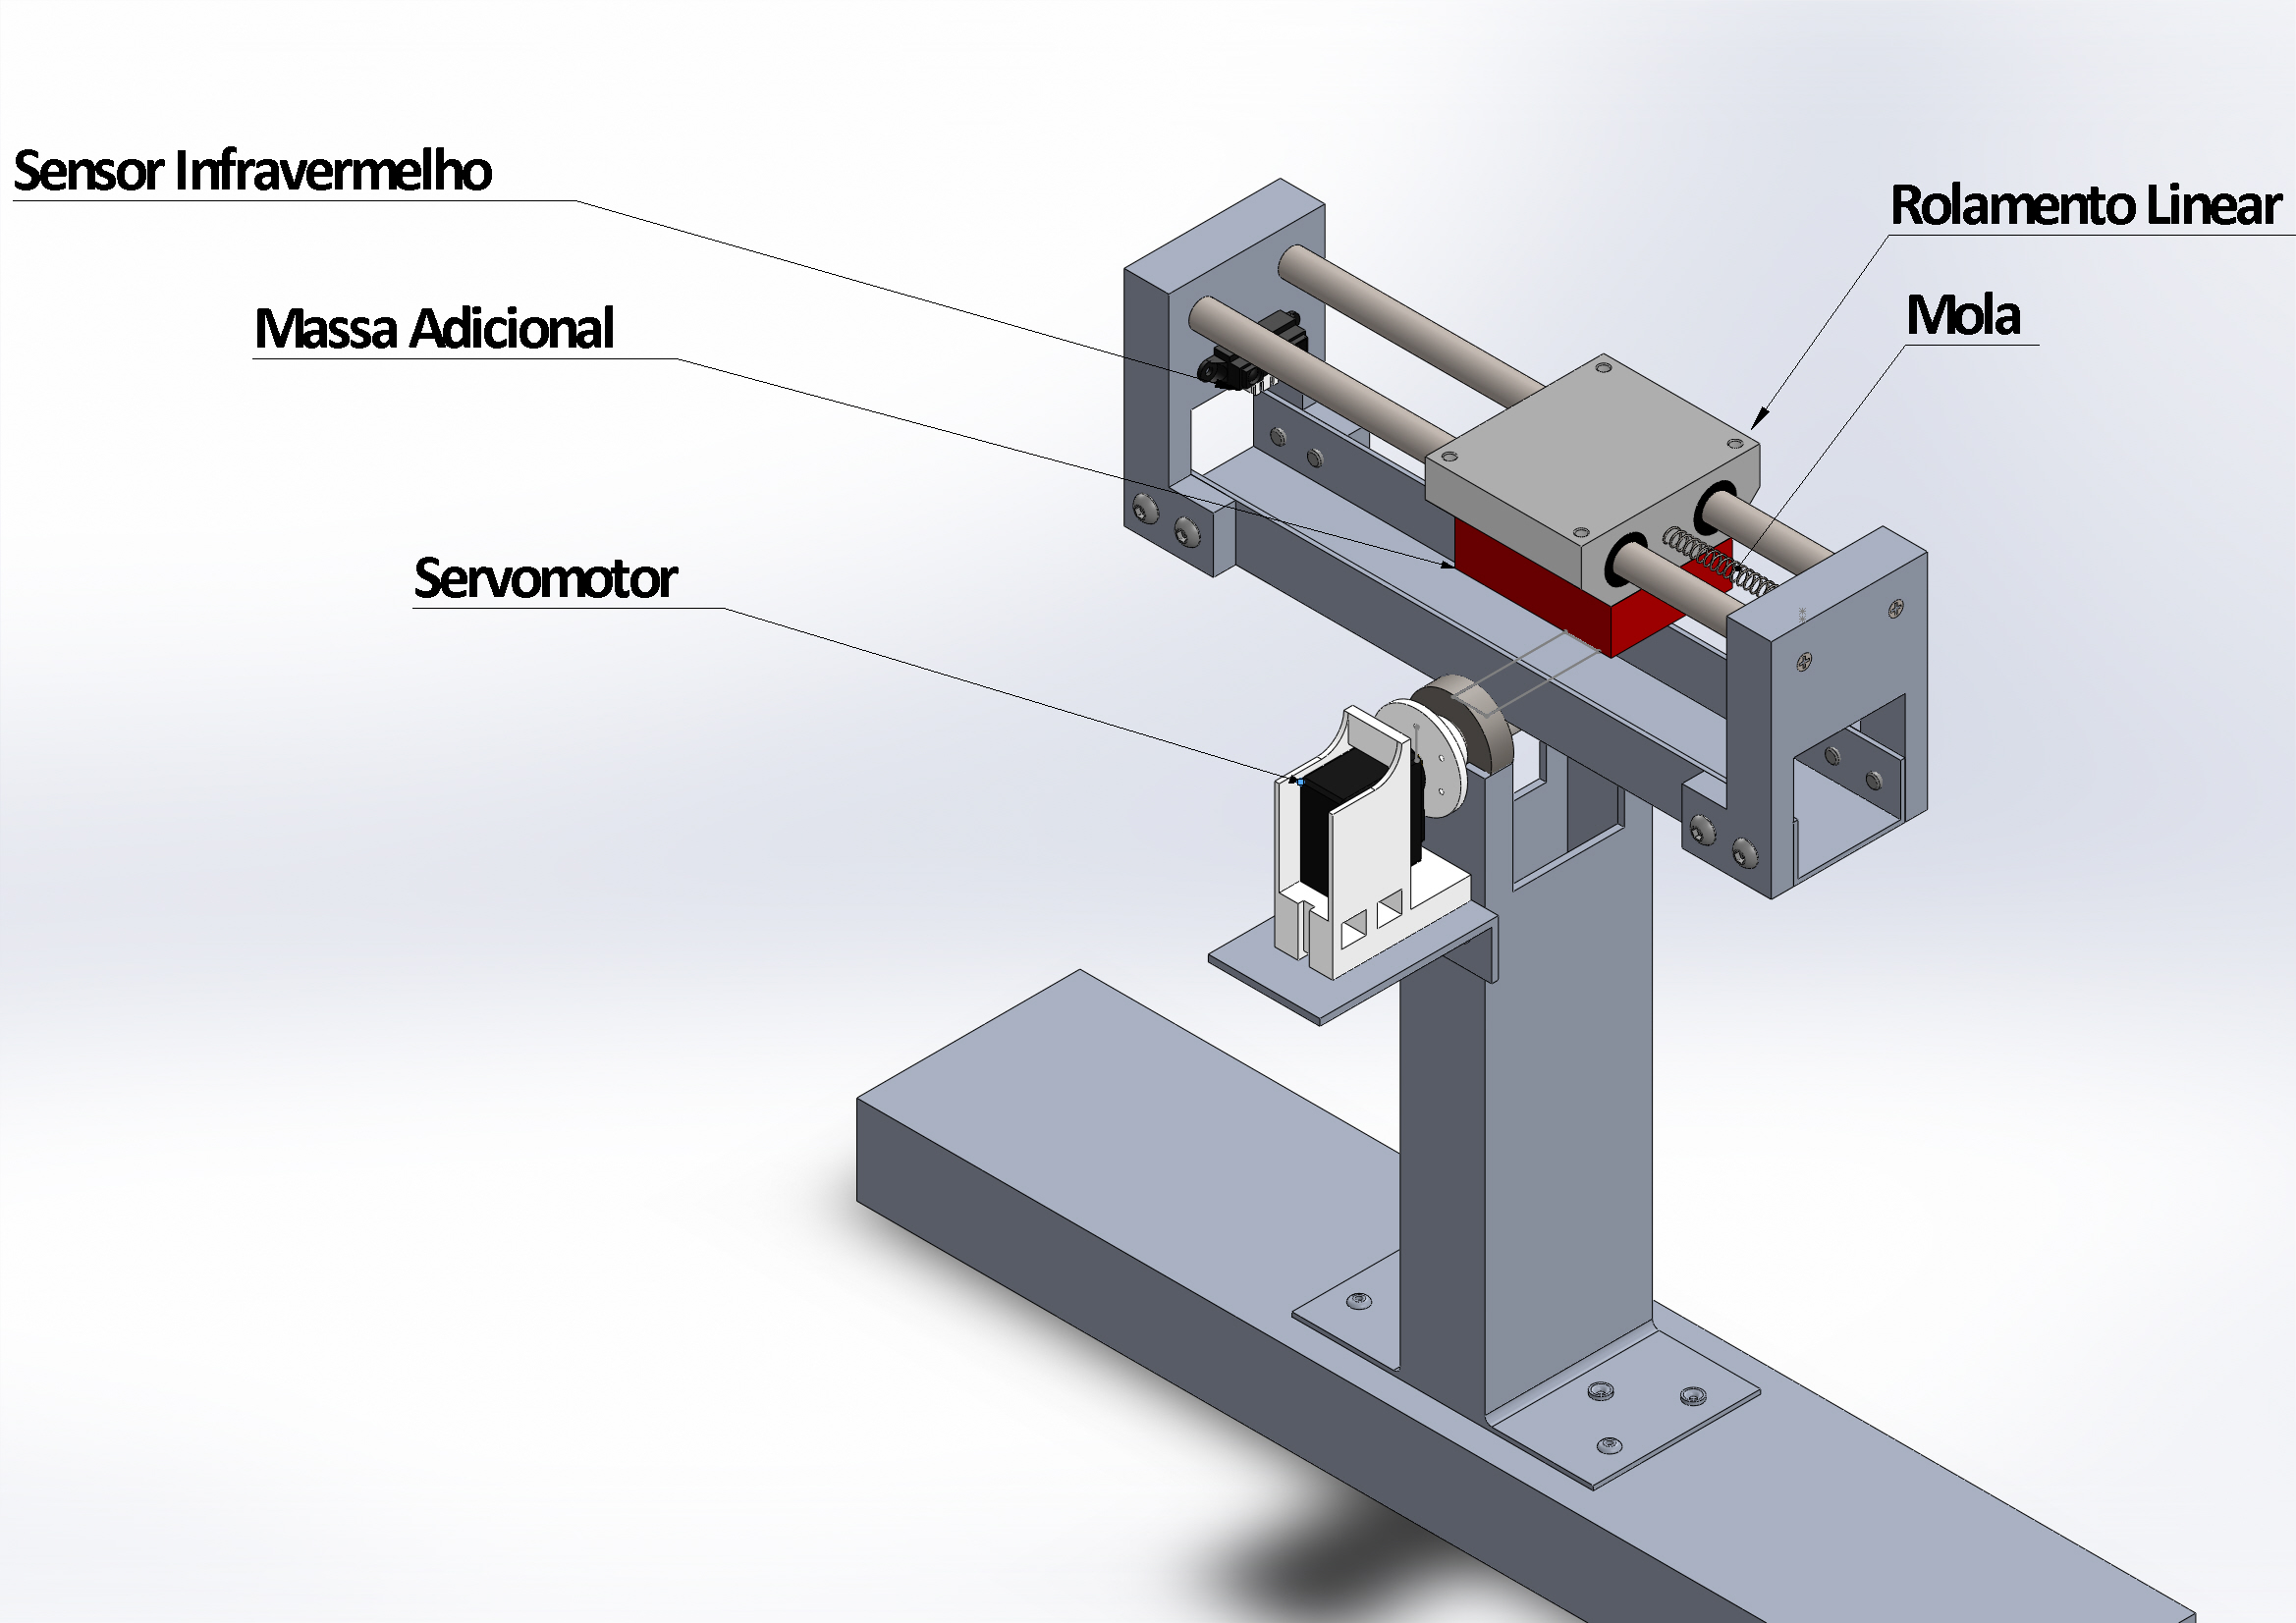
\includegraphics[width=0.9\linewidth]{planta}
  % texto que aparece abaixo da figura. O % no fim da linha anula a quebra de
  % linha, o que faz com que o \label fique junto com o caption, evitando erro
  % de offset quando o usuário clicar em um reflink no PDF. Eu uso inícios
  % padões em toda label: fig, eq, tbl, sec, subsec, chp... e recomendo que você
  % faça o mesmo.
  \caption{Sistema Massa-Mola}%
  \label{fig:smm1}
\end{figure}

Na Figura~\ref{fig:smm2} temos um exemplo de subfiguras.

\begin{figure}[ht!]
  \centering
  \subbottom[One]{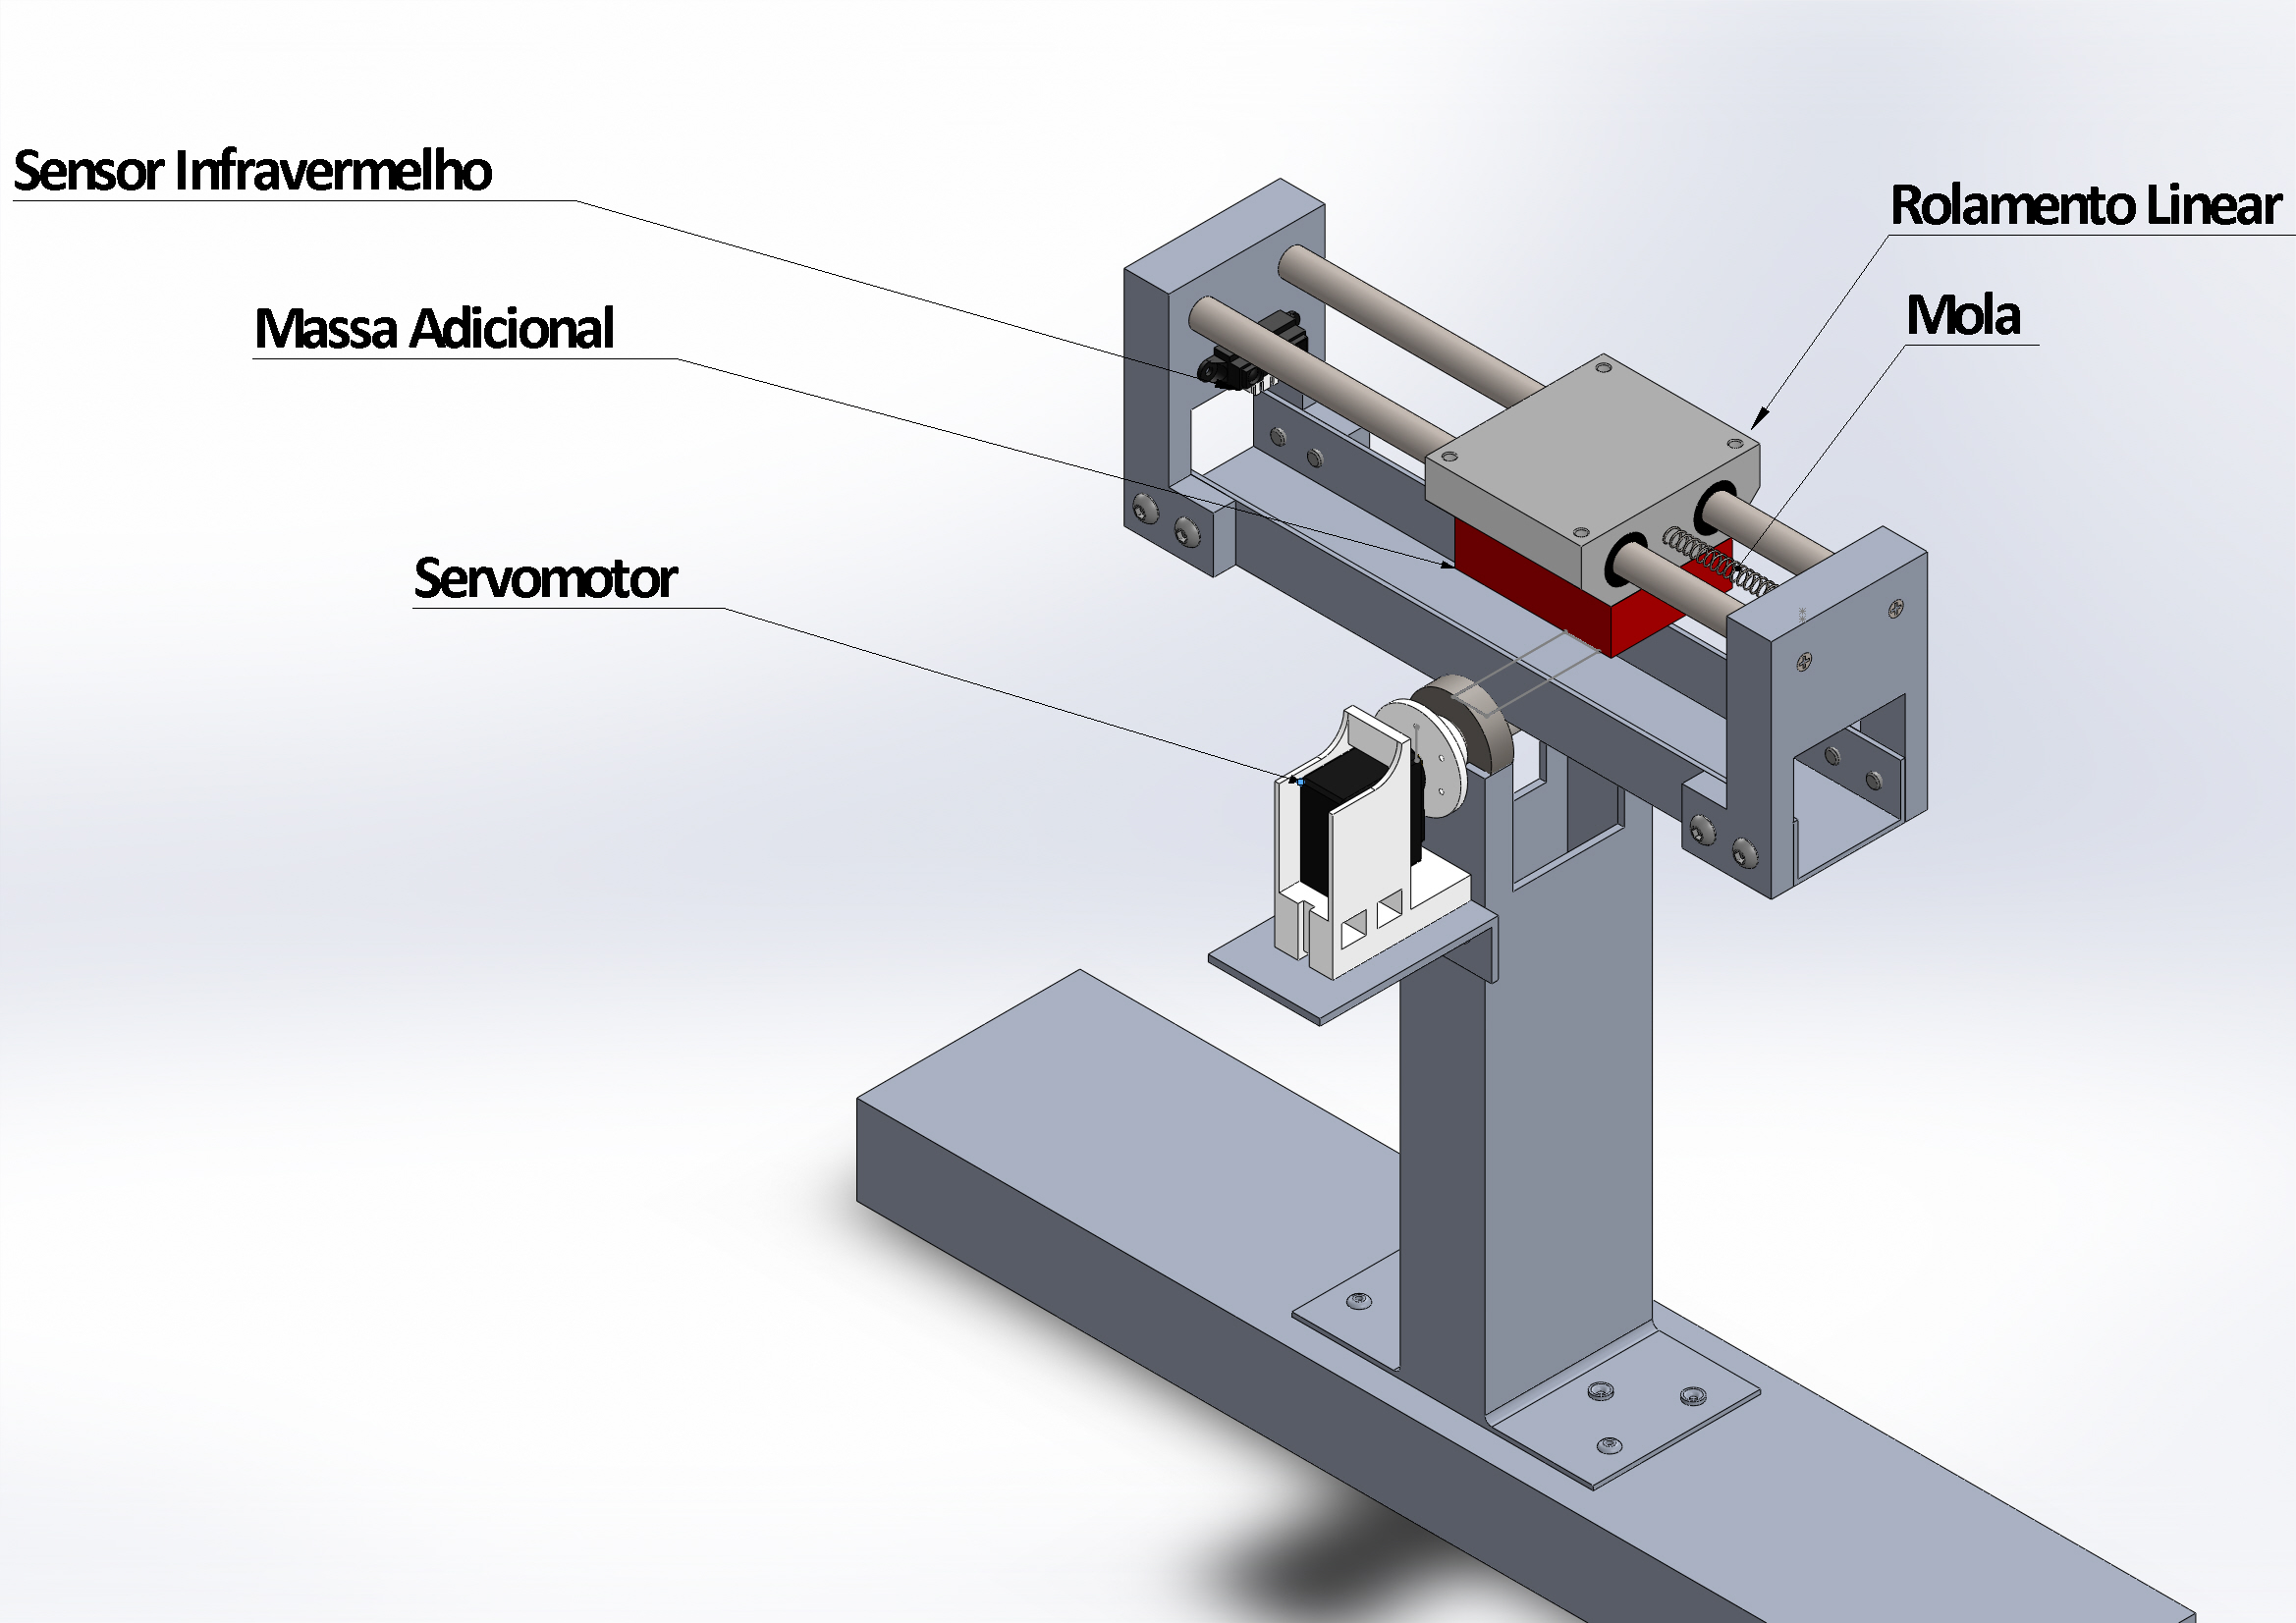
\includegraphics[width=0.4\linewidth]{planta}}\qquad
  \subbottom[Two]{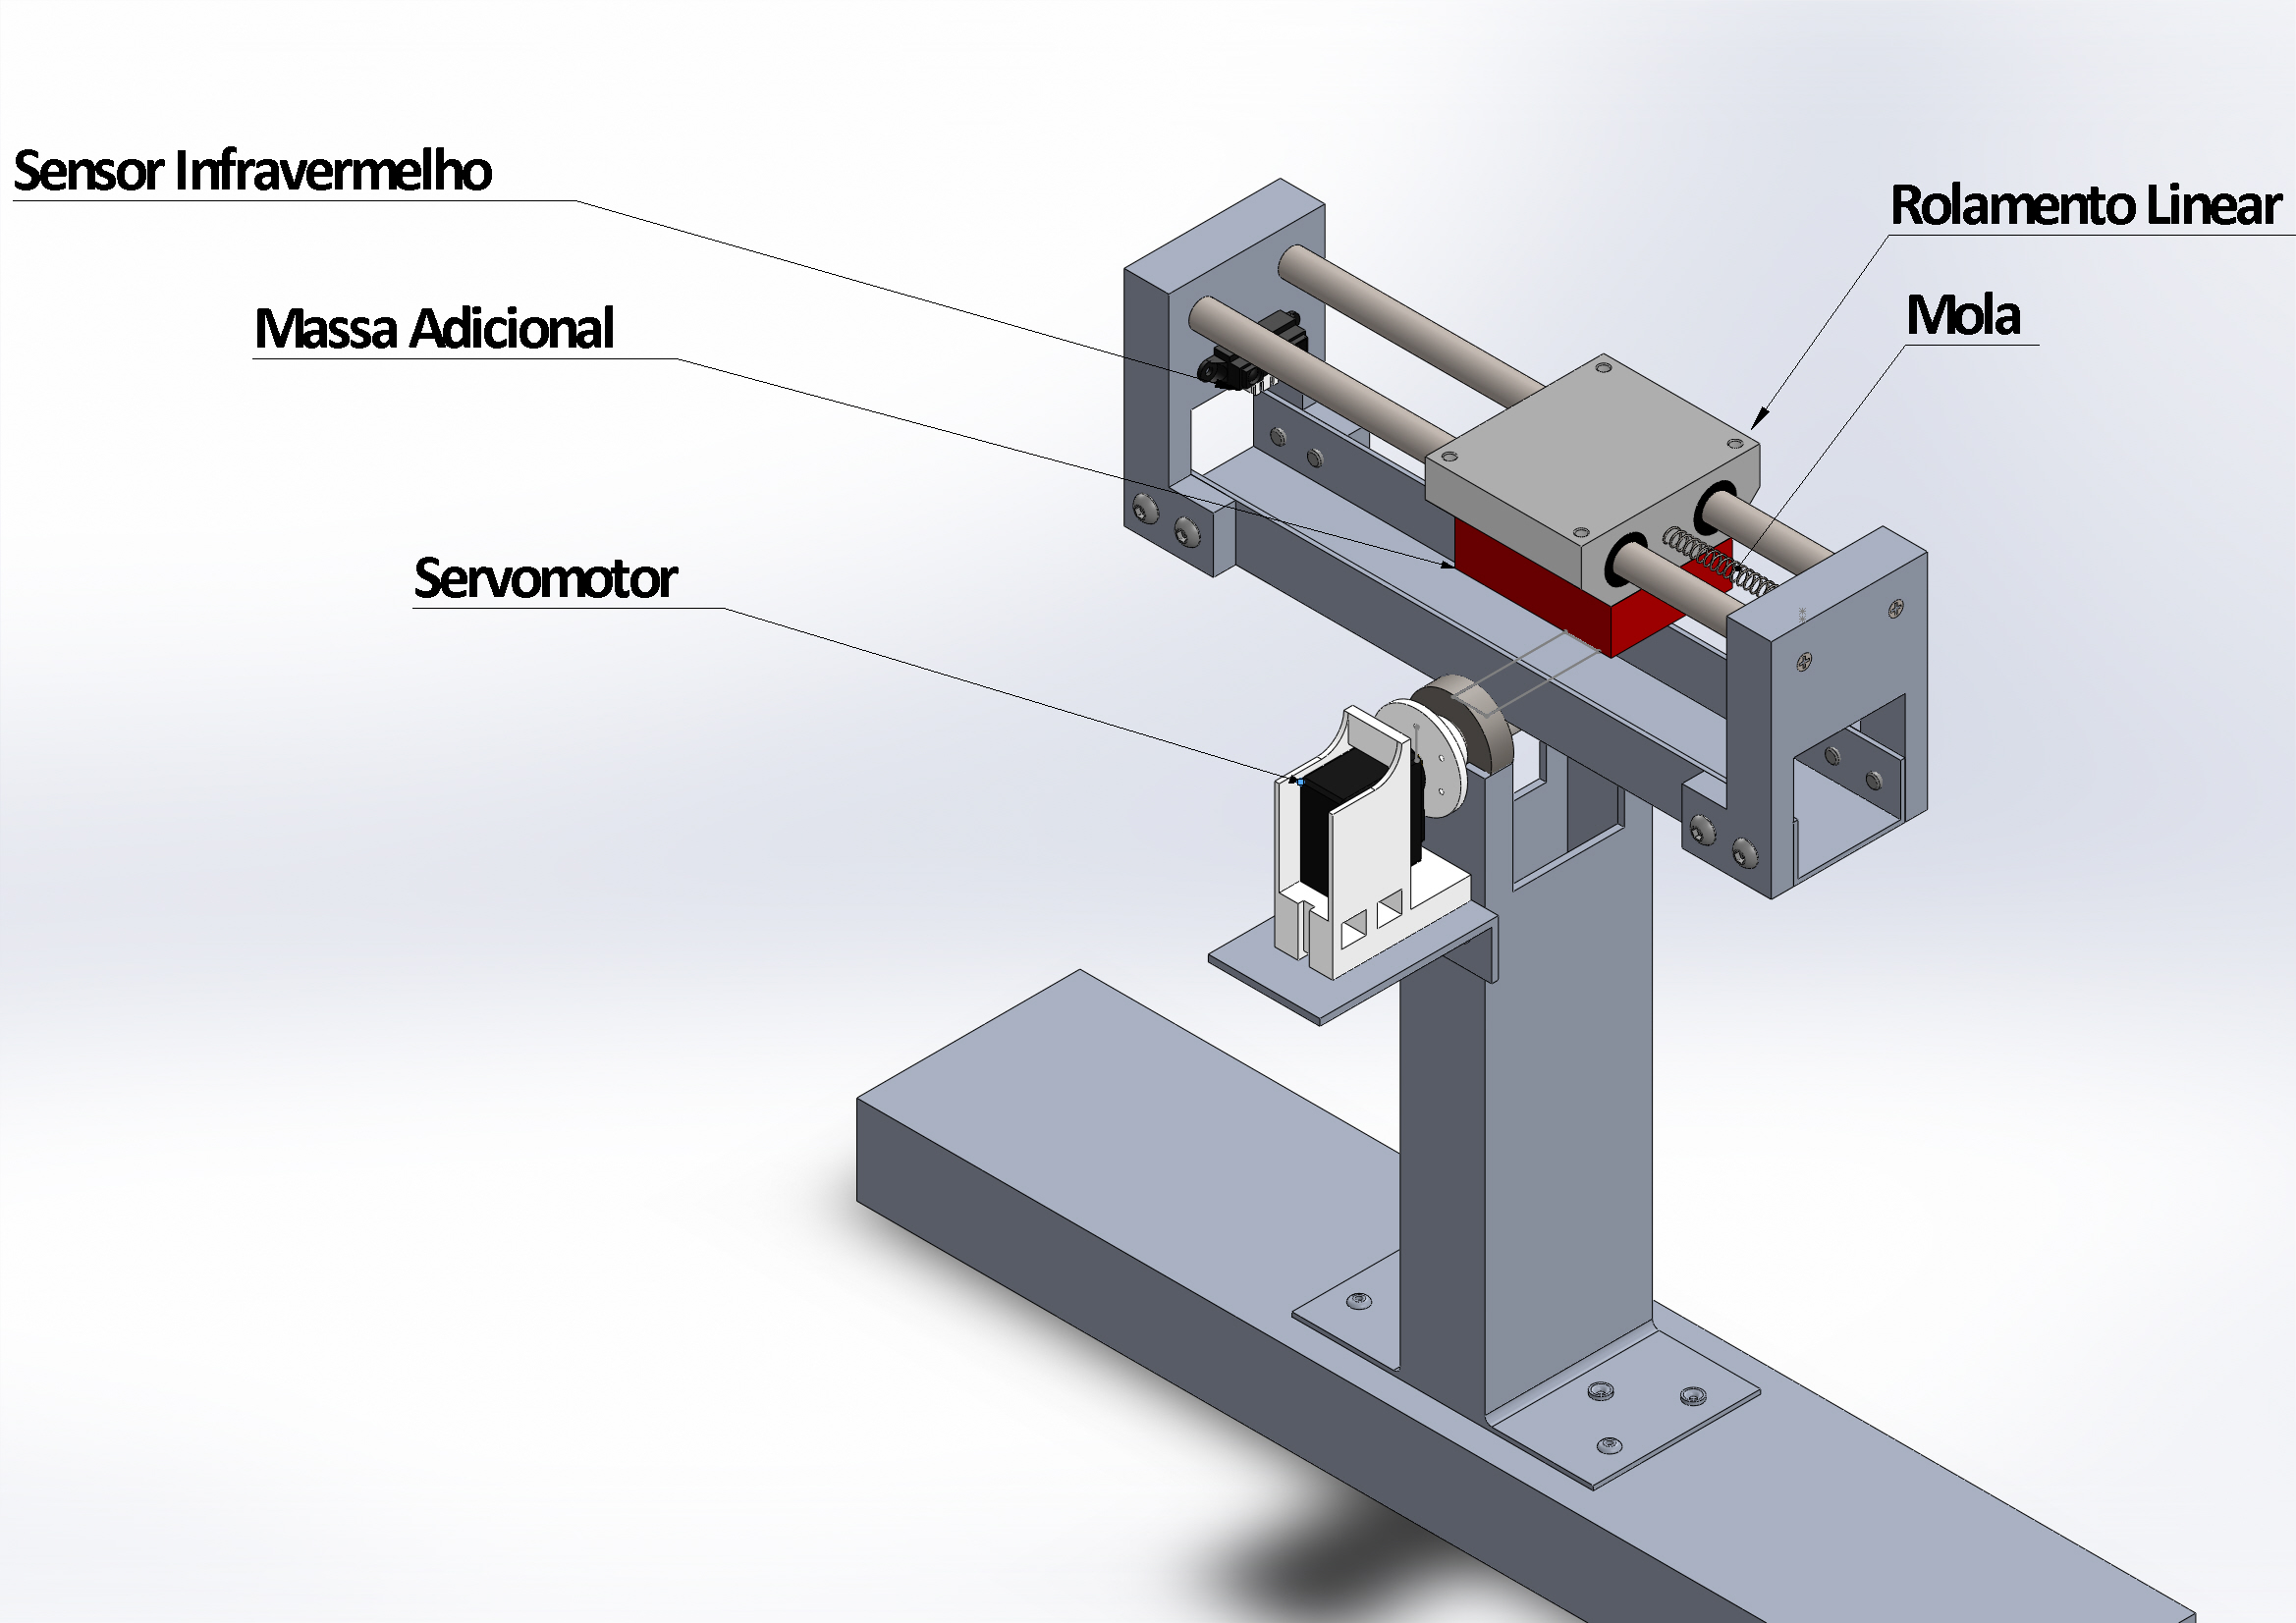
\includegraphics[width=0.4\linewidth]{planta}}
  \caption{Dois sistemas massa-mola.}%
  \label{fig:smm2}
\end{figure}

\FloatBarrier % impede que as figuras já definidas passem para a próxima seção.
% O Latex sempre tenta posicionar os floats (figura/tabelas) e o texto de forma
% eficiente quanto ao espaço, então em várias situações ele vai mandar a figura
% pra próxima página ou atravessar pra próxima seção. Se isso não é desejado,
% basta usar o \FloatBarrier que todos os floats declarados que ainda não foram
% posicionados serão posicionados nesse ponto. Se não entendeu, remova e veja a
% diferença no posicionamento das figuras e tabela em relação ao texto.

\section{Tabela}

A Tabela~\ref{tbl:exemplo} mostra como fazer uma tabela com ou sem linhas.

% Eu uso https://www.tablesgenerator.com pra gerar a tabela, e depois edito.
\begin{table}[ht!]
  \centering
  % Você deve fornecer um alinhamento para cada coluna. O símbolo | entre as
  % colunas indica que uma linha será desenhada.
  \begin{tabular}{l|cccc}
    \toprule
    Professor & Mecânica       & Eletrônica     & Controle       & Programação    \\ \midrule
    Lúcio     & \(\checkmark\) &                &                &                \\
    Valter    &                &                & \(\checkmark\) &                \\
    Thiago    &                &                &                & \(\checkmark\) \\
    Marlon    &                & \(\checkmark\) &                &                \\
    \bottomrule
  \end{tabular}
  \caption{Eixo de professores.}%
  \label{tbl:exemplo}
\end{table}
% Este exemplo mostra como usar top/mid/bottom rules e linhas verticais. No
% entanto, o povo do latex não recomenda usar isso dizendo que fica feio. No
% fim do dia o documento é seu, use ou não se quiser.
